\section{Алгоритм Рабина --- Карпа, алгоритм Кнута --- Морриса -- Пратта.  Структура данных «бор», алгоритм Ахо --- Корасик}

\subsection{Алгоритм Рабина --- Карпа}

Алгоритм Рабина --- Карпа предназначен для поиска подстроки в строке.
Наивный алгоритм поиска подстроки в строке работает за $O(n^2)$ в худшем случае --- слишком долго.
Чтобы ускорить этот процесс, можно воспользоваться методом хеширования.

\begin{definition}
    Пусть дана строка $s[0..n-1]$. Тогда \textbf{полиномиальным хешем} (англ. polynomial hash) строки $s$ называется число $h=hash(s[0..n-1])=p^0 s[0]+...+p^{n-1}s[n-1]$, где $p$ --- некоторое простое число, а $s[i]$ --- код $i$-го символа строки s.
\end{definition}

Проблему переполнения при вычислении хешей довольно больших строк можно решить так --- считать хеши по модулю $r=2^{64}$ (или $2^{32}$), чтобы модуль брался автоматически при переполнении типов.
Для работы алгоритма потребуется считать хеш подстроки $s[i..j]$.
Делать это можно следующим образом:

Рассмотрим хеш s[0..j]: $$hash(s[0..j])=s[0]+ps[1]+...+p^{i-1}s[i-1]+p^is[i]+...+p^{j-1}s[j-1]+p^js[j].$$
Разобьем это выражение на две части: $$hash(s[0..j])=(s[0]+ps[1]+...+p^{i-1}s[i-1])+(p^is[i]+...+p^{j-1}s[j-1]+p^js[j]).$$
Вынесем из последней скобки множитель $p^i$: $$hash(s[0..j])=(s[0]+ps[1]+...+p^{i-1}s[i-1])+p^i(s[i]+...+p^{j-i-1}s[j-1]+p^{j-i}s[j]).$$
Выражение в первой скобке есть не что иное, как хеш подстроки $s[0..i-1]$, а во второй --- хеш нужной нам подстроки $s[i..j]$.
Итак, мы получили, что: $$hash(s[0..j])=hash(s[0..i-1])+p^ihash(s[i..j]).$$
Отсюда получается следующая формула для $hash(s[i..j])$: $$hash(s[i..j])=(1/p^i)(hash(s[0..j])-hash(s[0..i-1])).$$

Однако, как видно из формулы, чтобы уметь считать хеш для всех подстрок, начинающихся с $i$, нужно предпосчитать все $p^i$ для $i \in [0..n-1]$.
Это займет много памяти.
Но поскольку нам нужны только подстроки размером $m$, мы можем подсчитать хеш подстроки $s[0..m-1]$, а затем пересчитывать хеши для всех $i \in [0..n-m]$ за $O(1)$ следующим образом: $$hash(s[i+1..i+m-1])=(hash(s[i..i+m-1])-p^{m-1}s[i])\mod r.$$
$$hash(s[i+1..i+m])=(p \cdot hash(s[i+1..i+m-1])+s[i+m])\mod r.$$
Получается: $$hash(s[i+1..i+m])=(p \cdot hash(s[i..i+m-1])-p^is[i]+s[i+m]) \mod r.$$

\subsubsection{Алгоритм}

Алгоритм начинается с подсчета $hash(s[0..m-1])$ и $hash(p[0..m-1])$, а также с подсчета $p^m$, для ускорения ответов на запрос.

Для $i \in [0..n-m]$ вычисляется $hash(s[i..i+m-1])$ и сравнивается с $hash(p[0..m-1])$.
Если они оказались равны, то образец $p$, скорее всего, содержится в строке $s$ начиная с позиции $i$, хотя возможны и ложные срабатывания алгоритма.
Если требуется свести такие срабатывания к минимуму или исключить вовсе, то применяют сравнение некоторых символов из этих строк, которые выбраны случайным образом, или применяют явное сравнение строк, как в наивном алгоритме поиска подстроки в строке.
В первом случае проверка произойдет быстрее, но вероятность ложного срабатывания, хоть и небольшая, останется.
Во втором случае проверка займет время, равное длине образца, но полностью исключит возможность ложного срабатывания.

Если требуется найти индексы вхождения нескольких образцов, или сравнить две строки --- выгоднее будет предпосчитать все степени $p$, а также хеши всех префиксов строки $s$.

\subsubsection{Псевдокод}

Приведем пример псевдокода, который находит все вхождения строки $w$ в строку $s$ и возвращает массив позиций, откуда начинаются вхождения.

\begin{minted}{c++}
vector<int> rabinKarp (s : string, w : string):
   vector<int> answer
   int n = s.length
   int m = w.length
   int hashS = hash(s[0..m - 1])
   int hashW = hash(w[0..m - 1])
   for i = 0 to n - m
        if hashS == hashW
             answer.add(i)
        hashS = (p * hashS - pm

 * hash(s[i]) + hash(s[i + m])) mod r // r — некоторое большое число, p — некоторое просто число
   return answer
\end{minted}

Новый хеш $hashS$ был получен с помощью быстрого пересчёта.
Для сохранения корректности алгоритма нужно считать, что $s[n+1]$ --- пустой символ.

\subsubsection{Время работы}

Изначальный подсчёт хешей выполняется за $O(m)$.
Каждая итерация выполняется за $O(1)$.
В цикле всего $n-m+1$ итераций.
Итоговое время работы алгоритма $O(n+m)$.

Однако если требуется исключить ложные срабатывания алгоритма полностью, т.е. придется проверить все полученные позиции вхождения на истинность, то в худшем случае итоговое время работы алгоритма будет $O(n \cdot m)$.

\subsection{Алгоритм Кнута --- Морриса --- Пратта}

Алгоритм Кнута --- Морриса --- Пратта (англ. Knuth–Morris–Pratt algorithm) --- алгоритм поиска подстроки в строке.

\subsubsection{Алгоритм}

Дана цепочка $T$ и образец $P$.
Требуется найти все позиции, начиная с которых $P$ входит в $T$.
Построим строку $S=P\#T$, где $\#$ --- любой символ, не входящий в алфавит $P$ и $T$.
Посчитаем на ней значение префикс-функции $p$.
Благодаря разделительному символу $\#$ выполняется $\forall i:p[i] \le |P|$.
Заметим, что по определению префикс-функции при $i>|P|$ и $p[i]=|P|$ подстроки длины $P$, начинающиеся с позиций 0 и $i-|P|+1$, совпадают.
Соберем все такие позиции $i-|P|+1$ строки $S$, вычтем из каждой позиции $|P|+1$, это и будет ответ.
Другими словами, если в какой-то позиции $i$ выполняется условие $p[i]=|P|$, то в этой позиции начинается очередное вхождение образца в цепочку.

\subsubsection{Псевдокод}

\begin{minted}{c}
int[] kmp(string P, string T):
   int pl = P.length
   int tl = T.length
   int[] answer
   int[] p = prefixFunction(P + "#" + T)
   int count = 0
   for i = 0 .. tl - 1
      if p[pl + i + 1] == pl
         answer[count++] = i - pl
   return answer
\end{minted}

\subsubsection{Время работы}

Префикс-функция от строки $S$ строится за $O(S)=O(P+T)$.
Проход цикла по строке $S$ содержит $O(T)$ итераций.
Суммарное время работы алгоритма оценивается как $O(P+T)$. 

\subsubsection{Оценка по памяти}

Предложенная реализация имеет оценку по памяти $O(P+T)$.
Оценки $O(P)$ можно добиться за счет запоминания значений префикс-функции для позиций в $S$, меньших $|P|+1$ (то есть до начала цепочки $T$).
Это возможно, так как значение префикс-функции не может превысить длину образца благодаря разделительному символу $\#$. 

\subsection{Структура данных «бор»}

\begin{definition}
    \textbf{Бор} (англ. trie, луч, нагруженное дерево) --- структура данных для хранения набора строк, представляющая из себя дерево с символами на рёбрах.
    Строки получаются последовательной записью всех символов, хранящихся на рёбрах между корнем бора и терминальной вершиной.
    Размер бора линейно зависит от суммы длин всех строк, а поиск в бору занимает время, пропорциональное длине образца. 
\end{definition}

\subsubsection{Пример}

Бор для набора образцов \{he, she, his, hers\}:

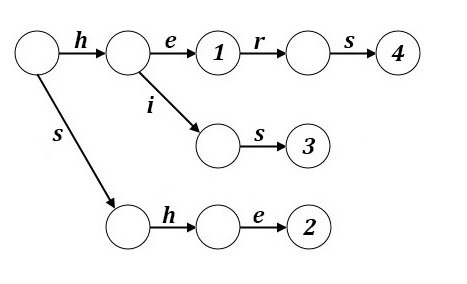
\includegraphics[]{img/9_1.jpg}

\subsubsection{Построение}

Введем следующие обозначения:

\begin{enumerate}
    \item $S$ --- используемый алфавит;
    \item $P={P_1,…,P_k}$ --- набор строк над $S$, называемый словарём;
    \item $n = \sum_{i = 1}^k |P_i|$ --- сумма длин строк.
\end{enumerate}

Бор храним как набор вершин, у каждой из которых есть метка, обозначающая, является ли вершина терминальной и указатели (рёбра) на другие вершины или на NULL.

\begin{minted}{c}
struct vertex:
    vertex next[|S|] 
    bool isTerminal
\end{minted}

\begin{enumerate}
    \item Создадим дерево из одной вершины (в нашем случае --- корня).
    \item Добавление элементов в дерево.
    Добавляем шаблоны $P_i$ один за другим.
    Следуем из корня по рёбрам, отмеченным буквами из $P_i$, пока возможно.
    Если $P_i$ заканчивается в $v$, сохраняем идентификатор $P_i$ (например, $i$) в $v$ и отмечаем вершину $v$ как терминальную.
    Если ребра, отмеченного очередной буквой $P_i$, нет, то создаем новое ребро и вершину для символа строки $P_i$.
\end{enumerate}

Построение занимает, очевидно, $O(|P_1|+...+|P_k|)=O(n)$ времени, так как поиск буквы, по которой нужно переходить, происходит за $O(1)$.
Поскольку на каждую вершину приходится $O(|S|)$ памяти, то использование памяти есть $O(n|S|)$. 

\subsection{Алгоритм Ахо --- Корасик.}

Пусть дан набор строк в алфавите размера $k$ суммарной длины $m$.
Необходимо найти для каждой строки все ее вхождения в текст.

\subsubsection{Шаг 1. Построение бора}

Строим бор из строк.
Построение выполняется за время $O(m)$, где $m$ --- суммарная длина строк.

\subsubsection{Шаг 2. Преобразование бора}

Обозначим за $[u]$ слово, приводящее в вершину $u$ в боре.
Узлы бора можно понимать как состояния автомата, а корень как начальное состояние.
Узлы бора, в которых заканчиваются строки, становятся терминальными.
Для переходов по автомату заведём в узлах несколько функций:

\begin{enumerate}
    \item $parent(u)$ — возвращает родителя вершины u;
    \item $\pi(u)=\delta(\pi(parent(u)),c)$ --- \textbf{суффиксная ссылка}, и существует переход из $parent(u)$ в $u$ по символу $c$;
    \item Функция перехода $\delta(u, c)=\begin{cases}
    v, \text{если из $u$ в $v$ ведёт символ $c$};\\
    root, \text{если $u$ --- корень и из него не исходит символ $c$};\\
    \delta(\pi(u), c), \text{иначе}.
    \end{cases}$
\end{enumerate}

Мы можем понимать рёбра бора как переходы в автомате по соответствующей букве.
Однако одними только рёбрами бора нельзя ограничиваться.
Если мы пытаемся выполнить переход по какой-либо букве, а соответствующего ребра в боре нет, то мы тем не менее должны перейти в какое-то состояние.
Для этого нам и нужны суффиксные ссылки.
Суффиксная ссылка $\pi(u)=v$, если $[v]$ --- максимальный суффикс $[u]$, $[v]\not=[u]$.
Функции перехода и суффиксные ссылки можно найти либо алгоритмом обхода в глубину с ленивыми вычислениями, либо с помощью алгоритма обхода в ширину. 

Из определений выше можно заметить два следующих факта:

\begin{itemize}
    \item функция перехода определена через суффиксную ссылку, а суффиксная ссылка — через функию переходов;
    \item для построения суффиксных ссылок небходимо знать информацию только выше по бору от текущей вершины до корня.
\end{itemize}

Это позволяет реализовать функции поиска переходов по символу и суффиксных ссылок ленивым образом при помощи взаимной рекурсии.

\subsubsection{Пример автомата Ахо-Корасик}

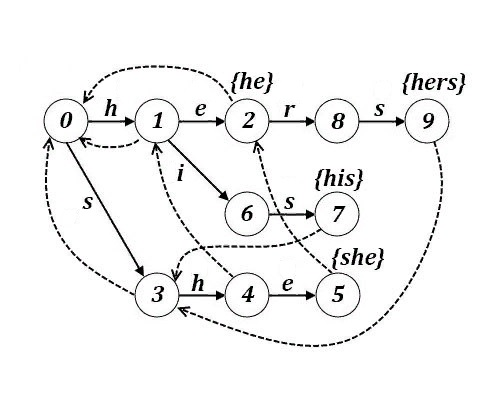
\includegraphics[]{img/9_2.jpg}

Пунктиром обозначены суффиксные ссылки.
Из вершин, для которых они не показаны, суффиксные ссылки идут в корень.

Суффиксная ссылка для каждой вершины $u$ --- это вершина, в которой оканчивается наидлиннейший собственный суффикс строки, соответствующей вершине $u$.
Единственный особый случай --- корень бора: для удобства суффиксную ссылку из него проведём в себя же.
Например, для вершины 5 с соответствующей ей строкой \textbf{she} максимальным подходящим суффиксом является строка \textbf{he}.
Видим, что такая строка заканчивается в вершине 2.
Следовательно суффиксной ссылкой вершины для 5 является вершина 2. 

\subsubsection{Шаг 3. Построение сжатых суффиксных ссылок}

При построении автомата может возникнуть такая ситуация, что ветвление есть не на каждом символе.
Тогда можно маленький бамбук заменить одним ребром.
Для этого и используются сжатые суффиксные ссылки.

$$up(u) = \begin{cases}
    \pi(u), \text{если $\pi(u)$ --- терминальная};\\
    \emptyset, \text{если $\pi(u)$ --- корень};\\
    up(\pi(u)), \text{иначе}.
\end{cases}$$

Здесь $up$ --- сжатая суффиксная ссылка, т.е. ближайшее допускающее состояние (терминал) перехода по суффиксным ссылкам.
Аналогично обычным суффиксным ссылкам, сжатые суффиксные ссылки могут быть найдены при помощи ленивой рекурсии.

\subsubsection{Использование автомата}

По очереди просматриваем символы текста.
Для очередного символа $c$ переходим из текущего состояния $u$ в состояние, которое вернёт функция $\delta(u,c)$.
Оказавшись в новом состоянии, отмечаем по сжатым суффиксным ссылкам строки, которые нам встретились, и их позицию (если требуется).
Если новое состояние является терминальным, то соответствующие ему строки тоже отмечаем.
